\newcommand{\TODO}[1]{\marginpar{\tiny TODO: #1}}

\DefineVerbatimEnvironment{code}{Verbatim}{frame=single}
%\DefineVerbatimEnvironment{icode}{Verbatim}{frame=none}
\newcommand{\icode}[1]{\texttt{#1}}

% Used in algorithms
\newcommand{\afor}{\textbf{for} {}}
\newcommand{\aif}{\textbf{if} {}}
\newcommand{\aelse}{\textbf{else} {}}
\newcommand{\seq}[1]{\left\langle{#1}\right\rangle}

% Boldface letters
\newcommand{\Ac}{\mathcal{A}}
\newcommand{\Bc}{\mathcal{B}}
\newcommand{\Cc}{\mathcal{C}}
\newcommand{\Dc}{\mathcal{D}}
\newcommand{\Lc}{\mathcal{L}}
\renewcommand{\AA}{\mathbf{A}}
\newcommand{\BB}{\mathbf{B}}
\newcommand{\CC}{\mathbf{C}}
\newcommand{\DD}{\mathbf{D}}
\newcommand{\EE}{\mathbf{E}}
\newcommand{\FF}{\mathbf{F}}
\newcommand{\II}{\mathbf{I}}
\newcommand{\MM}{\mathbf{M}}
\newcommand{\PP}{\mathbf{P}}
\renewcommand{\SS}{\mathbf{S}}
\newcommand{\VV}{\mathbf{V}}
\newcommand{\ee}{\mathbf{e}}
\newcommand{\ii}{\mathbf{i}}
\newcommand{\jj}{\mathbf{j}}
\newcommand{\kk}{\mathbf{k}}
\newcommand{\nn}{\mathbf{n}}
\newcommand{\uu}{\mathbf{u}}
\newcommand{\vv}{\mathbf{v}}
\newcommand{\ww}{\mathbf{w}}
\newcommand{\xx}{\mathbf{x}}
\newcommand{\ff}{\mathbf{f}}

\newcommand{\bpsi}{\bm{\psi}}
\newcommand{\bphi}{\bm{\phi}}
\newcommand{\bPsi}{\bm{\Psi}}
\newcommand{\bPhi}{\bm{\Phi}}

\newcommand{\mI}{\mathfrak{I}}
%\newcommand{\mI}{\mathcal{I}}

\newcommand{\Ic}{\mathcal{I}}

%\newcommand{\llbracket}{\left[}
%\newcommand{\rrbracket}{\right]}

%\DeclareMathOperator{\spanop}{span}

\newcommand{\mop}[1]{\operatorname{#1}}
\newcommand{\spans}[1]{\mop{span}\left\{ #1 \right\}}

%//////////////////////////////////////////////////////////////////////////////
\fenicschapter{UFL: A Finite Element Form Language}
              {UFL: A Finite Element Form Language}
              {Martin Sandve Aln\ae{}s}
              {alnes-1}
%\\\\\\\\\\\\\\\\\\\\\\\\\\\\\\\\\\\\\\\\\\\\\\\\\\\\\\\\\\\\\\\\\\\\\\\\\\\\\\

\index{Unified Form Language}
\index{\ufl{}}
\index{variational form}
\index{weak form}
\index{functional}
\index{form language}
\index{domain specific language}

\editornote{Sort out what to do with all UFL specific macros and bold math fonts.}

The Unified Form Language -- \ufl{}~\cite{manual:ufl,www:ufl} -- is a
domain specific language for the declaration of finite element
discretizations of variational forms and functionals. More precisely,
the language defines a flexible user interface for defining finite
element spaces and expressions for weak forms in a notation close to
mathematical notation.

The \fenics{} project~\cite{DupHof2003,www:fenics,Log2007} provides a framework for
building applications for solving partial differential equations (PDEs).
\ufl{} is one of the core components of this framework.
It defines the language you \emph{express} your PDEs in.
It is the input language and front-end of the form compilers
\ffc{}~\cite{KirLog2006,KirLog2007,manual:ffc,www:ffc,OelLog2008,OelWel2009}
and \sfc{}~\cite{www:syfi,manual:syfi}.  The \ufl{} implementation
provides algorithms that the form compilers can use to simplify the
compilation process.  The output from these form compilers is
\ufc{}~\cite{www:ufc,manual:ufc,AlnLog2009} conforming
C++~\cite{Str1997} code. This code can be used with the C++ library
\dolfin{}\footnote{Note that in \pydolfin{}, some parts of \ufl{} is
wrapped to blend in with other software components and make the
compilation process hidden from the user.  This is not discussed
here.}~\cite{LogWel2009,www:dolfin,manual:dolfin} to efficiently
assemble linear systems and compute solution to PDEs.

The combination of domain specific languages and symbolic computing
with finite element methods has been pursued from other angles in
several other projects.  Sundance~\cite{Lon03,Lon04a,www:sundance}
implements a symbolic engine directly in C++ to define variational
forms, and has support for automatic differentiation.  The
Life~\cite{Pru2006a,Pru2006b} project uses a domain specific language
embedded in C++, based on expression template techniques to specify
variational forms.  SfePy~\cite{www:sfepy} uses SymPy as a symbolic
engine, extending it with finite element methods.
GetDP~\cite{DulGeu2005,www:getdp} is another project using a domain
specific language for variational forms.  The Mathematica package
AceGen~\cite{Kor1997,Kor2002} uses the symbolic capabilities of
Mathematica to generate efficient code for finite element methods.
All these packages have in common a focus on high level descriptions
of partial differential equations to achive higher human efficiency in
the development of simulation software.

\ufl{} almost resembles a library for symbolic computing,
but its scope, goals and priorities are different from generic
symbolic computing projects such as GiNaC~\cite{www:ginac,BauFri2000},
swiginac~\cite{www:swiginac} and SymPy~\cite{www:sympy}.  Intended as
a domain specific language and form compiler frontend,
\ufl{} is not suitable for large scale symbolic computing.

This chapter is intended both for the \fenics{} user who wants to
learn how to express her equations, and for other \fenics{} developers
and technical users who wants to know how \ufl{} works on the inside.
Therefore, the sections of this chapter are organized with an
increasing amount of technical details.
Sections~\ref{ufl:sec:overview}-\ref{ufl:sec:formtransformations} give
an overview of the language as seen by the end-user and is intended
for all audiences.
Sections~\ref{ufl:sec:representation}-\ref{ufl:sec:implementation}
explain the design of the implementation and dive into some
implementation details.  Many details of the language has to be
omitted in a text such as this, and we refer to the \ufl{}
manual~\cite{manual:ufl} for a more thorough description. Note that
this chapter refers to \ufl{} version 0.3, and both the user interface
and the implementation may change in future versions.

Starting with a brief overview, we mention the main design goals for
\ufl{} and show an example implementation of a non-trivial PDE in
Section~\ref{ufl:sec:overview}.  Next we will look at how to define
finite element spaces in Section~\ref{ufl:sec:elements}, followed by
the overall structure of forms and their declaration in
Section~\ref{ufl:sec:forms}.  The main part of the language is
concerned with defining expressions from a set of data types and
operators, which are discussed in Section~\ref{ufl:sec:defexpr}.
Operators applying to entire forms is the topic of
Section~\ref{ufl:sec:formtransformations}.

The technical part of the chapter begins with
Section~\ref{ufl:sec:representation} which discusses the
representation of expressions.  Building on the notation and data
structures defined there, how to compute derivatives is discussed in
Section~\ref{ufl:sec:ad}.  Some central internal algorithms and key
issues in their implementation are discussed in
Section~\ref{ufl:sec:algorithms}.  Implementation details, some of
which are specific to the programming language
Python~\cite{www:python}, is the topic of
Section~\ref{ufl:sec:implementation}.  Finally,
Section~\ref{ufl:sec:future} discusses future prospects of the \ufl{}
project.

%==============================================================================
%\clearpage{}
\section{Overview} \label{ufl:sec:overview}

%------------------------------------------------------------------------------
\subsection{Design goals} \label{ufl:sec:goals}
\ufl{} is a unification, refinement and reimplementation of
the form languages used in previous versions of \ffc{} and \sfc{}.
The development of this language has been motivated by several
factors, the most important being:
\begin{itemize}
\item A richer form language, especially for expressing nonlinear PDEs.
\item Automatic differentiation of expressions and forms.
\item Improving the performance of the form compiler technology to handle more complicated equations efficiently.
\end{itemize}
\ufl{} fulfils all these requirements, and by this it represents
a major step forward in the capabilities of the \fenics{} project.

Tensor algebra and index notation support is modeled after the \ffc{}
form language and generalized further. Several nonlinear operators and
functions which only \sfc{} supported before have been included in the
language.  Differentiation of expressions and forms has become an
integrated part of the language, and is much easier to use than the
way these features were implemented in \sfc{} before.  In summary,
\ufl{} combines the best of \ffc{} and \sfc{} in one unified form
language and adds additional capabilities.

The efficiency of code generated by the new generation of form
compilers based on \ufl{} has been verified to match previous form
compiler benchmarks~\cite{AlnMar2009,OelWel2009}.  The form
compilation process is now fast enough to blend into the regular
application build process.  Complicated forms that previously required
too much memory to compile, or took tens of minutes or even hours to
compile, now compiles in seconds with both \sfc{} and \ffc{}.

%------------------------------------------------------------------------------
\subsection{Motivational example} \label{ufl:sec:example}
%~\cite{AlnMar2007}. % MekIT
%\TODO{Citations on hyperelasticity.}
One major motivating example during the initial development of \ufl{}
has been the equations for elasticity with large deformations.  In
particular, models of biological tissue use complicated hyperelastic
constitutive laws with anisotropies and strong nonlinearities.  To
implement these equations with \fenics{}, all three design goals
listed above had to be adressed.  Below, one version of the
hyperelasticity equations and their corresponding \ufl{}
implementation is shown.  Keep in mind that this is only intended as
an illustration of the close correspondence between the form language
and the natural formulation of the equations.  The meaning of
equations is not necessary for the reader to understand.  Note that
many other examples are distributed together with \ufl{}.

In the formulation of the hyperelasticity equations presented here,
the unknown function is the displacement vector field $\uu$.  The
material coefficients $c_1$ and $c_2$ are scalar constants.  The
second Piola-Kirchoff stress tensor $\SS$ is computed from the strain
energy function $W(\CC)$. $W$ defines the constitutive law, here a
simple Mooney-Rivlin law. The equations relating the displacement and
stresses read:
\begin{align}
\begin{split}
\FF   &=  \II + (\nabla \uu)^T, \\
\CC   &=  \FF^T\FF, \\
I_C   &=  \mop{tr}(\CC), \\
II_C  &=  \frac 1 2 (\mop{tr}(\CC)^2 - \mop{tr}(\CC\CC)), \\
W     &=  c_1(I_C - 3) + c_2(II_C - 3), \\
\SS   &=  2\frac{\partial W}{\partial\CC}, \\
\PP   &=  \FF\SS.
\end{split}
\end{align}
Approximating the displacement field as $\uu = \sum_k u_k \bphi^1_k$,
the weak forms of the equations are as follows (ignoring boundary conditions):
\begin{align}
L(\bphi^0; \uu, c_1, c_2) &= \int_\Omega \PP : (\nabla\bphi^0)^T \dx, \\
a(\bphi^0, \bphi^1_k; \uu, c_1, c_2) &= \frac{\partial L}{\partial u_k}.
\end{align}
% \quad \forall \bphi^0 \in V_h^0
\begin{figure}\label{ufl:fig:hypcode}
\begin{code}
# Finite element spaces
cell = tetrahedron
element = VectorElement("CG", cell, 1)

# Form arguments
phi0 = TestFunction(element)
phi1 = TrialFunction(element)
u = Function(element)
c1 = Constant(cell)
c2 = Constant(cell)

# Deformation gradient Fij = dXi/dxj
I = Identity(cell.d)
F = I + grad(u).T

# Right Cauchy-Green strain tensor C with invariants
C = variable(F.T*F)
I_C = tr(C)
II_C = (I_C**2 - tr(C*C))/2

# Mooney-Rivlin constitutive law
W = c1*(I_C-3) + c2*(II_C-3)

# Second Piola-Kirchoff stress tensor
S = 2*diff(W, C)

# Weak forms
L = inner(F*S, grad(phi0).T)*dx
a = derivative(L, u, phi1)
\end{code}
\caption{\ufl{} implementation of hyperelasticity equations with a Mooney-Rivlin material law.}
\end{figure}
Figure~\ref{ufl:fig:hypcode} shows an implementation of these
equations in \ufl{}.  Notice the close relation between the
mathematical notation and the \ufl{} source code. In particular, note
the automated differentiation of both the constitutive law and the
residual equation. This means a new material law can be implemented by
simply changing $W$, the rest is automatic.  In the following
sections, the notation, definitions and operators used in this
implementation are explained.

%==============================================================================
%\clearpage{}
\section{Defining finite element spaces} \label{ufl:sec:elements}
\index{finite element}
\index{finite element space}
\index{Lagrange element}
\index{discontinuous Lagrange element}
\index{\icode{FiniteElement}}
\index{\icode{VectorElement}}
\index{\icode{TensorElement}}
\index{\icode{MixedElement}}
A polygonal cell is defined by a basic shape and a
degree\footnote{Note that at the time of writing, the other components
of \fenics{} does not yet handle higher degree cells.}, and is
declared
\begin{code}
cell = Cell(shape, degree)
\end{code}
\ufl{} defines a set of valid polygonal cell shapes:
``interval'', ``triangle'', ``tetrahedron'', ``quadrilateral'', and ``hexahedron''.
Linear cells of all basic shapes are predefined and can be used instead by writing
\begin{code}
cell = tetrahedron
\end{code}
In the rest of this chapter, a variable name \icode{cell} will be used
where any cell is a valid argument, to make the examples dimension
independent wherever possible.

\ufl{} defines syntax for \emph{declaring} finite element spaces,
but does not know anything about the actual polynomial basis or
degrees of freedom. The polynomial basis is selected implicitly by
choosing among predefined basic element families and providing a
polynomial degree, but
\ufl{} only assumes that there \emph{exists} a basis
with a fixed ordering for each finite element space $V_h$, i.e.
\begin{align}
V_h = \spans{\phi_j}_{j=1}^{n}.
\end{align}
Basic scalar elements can be combined to form vector elements or
tensor elements, and elements can easily be combined in arbitrary
mixed element hierarchies.

The set of predefined\footnote{Form compilers can register additional
element families.}  element family names in \ufl{} includes
``Lagrange'' (short name ``CG''), representing scalar Lagrange finite
elements (continuous piecewise polynomial functions), ``Discontinuous
Lagrange'' (short name ``DG''), representing scalar discontinuous
Lagrange finite elements (discontinuous piecewise polynomial
functions), and a range of other families that can be found in the
manual.  Each family name has an associated short name for
convenience.  To print all valid families to screen from Python, call
\icode{show\_elements()}.

The syntax for declaring elements is best explained with some
examples.
\begin{code}
cell = tetrahedron

P = FiniteElement("Lagrange", cell, 1)
V = VectorElement("Lagrange", cell, 2)
T = TensorElement("DG", cell, 0, symmetry=True)

TH = V + P
ME = MixedElement(T, V, P)
\end{code}
In the first line a polygonal cell is selected from the set of
predefined linear cells.  Then a scalar linear Lagrange element
\icode{P} is declared, as well as a quadratic vector Lagrange element
\icode{V}.  Next a symmetric rank 2 tensor element \icode{T} is
defined, which is also piecewise constant on each cell.  The code
pproceeds to declare a mixed element \icode{TH}, which combines the
quadratic vector element \icode{V} and the linear scalar element
\icode{P}. This element is known as the Taylor-Hood element.  Finally
another mixed element with three sub elements is declared. Note that
writing \icode{T + V + P} would not result in a mixed element with
three direct sub elements, but rather
\icode{MixedElement(MixedElement(T + V), P)}.

%==============================================================================
%\clearpage{}
\section{Defining forms}
\label{ufl:sec:forms}
\index{\icode{Form}}
\index{\icode{Integral}}
\index{\icode{Measure}}
\index{forms}
\index{integrals}
\index{interior measure}
\index{cell integral}
\index{boundary measure}
\index{exterior facet integral}
\index{boundary measure}
\index{interior facet integral}

Consider Poisson's equation with two different boundary
conditions on $\partial\Omega_0$ and $\partial\Omega_1$,
\begin{align}
a(v, u; w) &= \int_\Omega w \nabla u \cdot \nabla v \dx, \\
L(v; f, g, h) &= \int_\Omega f v \dx + \int_{\partial\Omega_0} g^2 v \ds + \int_{\partial\Omega_1} h v \ds.
\end{align}
These forms can be expressed in UFL as
\begin{code}
a = dot(grad(u), grad(v))*dx
L = f*v*dx + g**2*v*ds(0) + h*v*ds(1)
\end{code}
where multiplication by the measures \icode{dx}, \icode{ds(0)} and \icode{ds(1)}
represent the integrals $\int_{\Omega_0} (\cdot) \dx$,
$\int_{\partial\Omega_0} (\cdot) \ds$,
and $\int_{\partial\Omega_1} (\cdot) \ds$
respectively.

Forms expressed in \ufl{} are intended for finite element discretization
followed by compilation to efficient code for computing the element tensor.
Considering the above example, the bilinear form $a$ with one coefficient
function $w$ is assumed to be evaluated at a later point with a
range of basis functions and the coefficient function fixed, that is
\begin{align}
V_h^1 &= \spans{\phi_k^1}, \quad V_h^2 = \spans{\phi_k^2}, \quad V_h^3 = \spans{\phi_k^3}, \\
w &= \sum_{k=1}^{|V^2_h|} w_k \phi_k^3, \quad \{ w_k \} \mbox{ given}, \\
A_{ij} &= a(\phi_i^1, \phi_j^2; w),
    \quad i = 1,\ldots,|V^1_h|, \quad j = 1,\ldots,|V^2_h| . \label{ufl:eq:Aij}
\end{align}

In general, \ufl{} is designed to express forms of the following generalized form:
\begin{align} \label{ufl:eq:form_integrals}
    a(&\phi^1, \ldots, \phi^r; w^1, \ldots,  w^n) =
           \sum_{k=1}^{n_c} \int_{\Omega_k}          I^c_k \dx
         + \sum_{k=1}^{n_e} \int_{\partial\Omega_k}  I^e_k \ds
         + \sum_{k=1}^{n_i} \int_{\Gamma_k}          I^i_k \dS.
\end{align}
Most of this chapter deals with ways to define the integrand
expressions $I^c_k$, $I^e_k$ and $I^i_k$.  The rest of the notation
will be explained below.

The form arguments are divided in two groups, the basis functions
$\phi^1,\ldots,\phi^r$ and the coefficient functions $w^1,\ldots,w^n$.
All $\{ \phi^k \}$ and $\{ w^k \}$ are functions in some discrete
function space with a basis.  Note that the actual basis functions $\{
\phi_j^k \}$ and the coefficients $\{ w_k \}$ are never known to
\ufl{}, but we assume that the ordering of the basis for each finite
element space is fixed. A fixed ordering only matters when
differentiating forms, explained in Section~\ref{ufl:sec:ad}.

Each term of a valid form expression must be a scalar-valued
expression integrated exactly once, and they must be linear in $\{
\phi^k \}$.  Any term may have nonlinear dependencies on coefficient
functions.  A form with one or two basis function arguments ($r=1,2$)
is called a linear or bilinear form respectively, ignoring its
dependency on coefficient functions. These will be assembled to
vectors and matrices when used in an application.  A form depending
only on coefficient functions ($r=0$) is called a functional, since it
will be assembled to a real number.

The entire domain is denoted $\Omega$, the external boundary is
denoted $\partial\Omega$, while the set of interior facets of the
triangulation is denoted $\Gamma$. Sub domains are marked with a
suffix, e.g., $\Omega_k \subset \Omega$. As mentioned above,
integration is expressed by multiplication with a measure, and \ufl{}
defines the measures \icode{dx}, \icode{ds} and \icode{dS}.  In
summary, there are three kinds of integrals with corresponding \ufl{}
representations
\begin{itemize}
\item $\int_{        \Omega_k} (\cdot) \dx$ $\leftrightarrow$  $(\cdot)$\icode{*dx(k)}, called a \emph{cell integral},
\item $\int_{\partial\Omega_k} (\cdot) \ds$ $\leftrightarrow$  $(\cdot)$\icode{*ds(k)}, called an \emph{exterior facet integral},
\item $\int_{        \Gamma_k} (\cdot) \dS$ $\leftrightarrow$  $(\cdot)$\icode{*dS(k)}, called an \emph{interior facet integral},
\end{itemize}
Defining a different quadrature order for
each term in a form can be achieved by attaching
meta data to measure objects, e.g.,
\begin{code}
dx02 = dx(0, { "integration_order": 2 })
dx14 = dx(1, { "integration_order": 4 })
dx12 = dx(1, { "integration_order": 2 })
L = f*v*dx02 + g*v*dx14 + h*v*dx12
\end{code}
Meta data can also be used to override other form compiler specific
options separately for each term. For more details on
this feature see the manuals of \ufl{} and the form compilers.


%==============================================================================
%\clearpage{}
\section{Defining expressions}
\label{ufl:sec:defexpr}
\index{\icode{Terminal}}
\index{\icode{Identity}}
\index{atomic value}
\index{terminal value}
\index{identity matrix}
\index{spatial coordinates}
\index{facet normal}
\index{form argument}
\index{basis function}
\index{coefficient function}

Most of \ufl{} deals with how to declare expressions such as the
integrand expressions in Equation~\ref{ufl:eq:form_integrals}.  The
most basic expressions are terminal values, which do not depend on
other expressions.  Other expressions are called operators, which are
discussed in sections
\ref{ufl:sec:indexnotation}-\ref{ufl:sec:conditionals}.

Terminal value types in \ufl{} include form arguments (which is the
topic of Section~\ref{ufl:sec:arguments}), geometric quantities, and
literal constants.  Among the literal constants are scalar integer and
floating point values, as well as the $d$ by $d$ identity matrix
\icode{I = Identity(d)}.  To get unit vectors, simply use rows or
columns of the identity matrix, e.g., \icode{e0 = I[0,:]}.  Similarly,
\icode{I[i,j]} represents the Dirac delta function $\delta_{ij}$ (see
Section~\ref{ufl:sec:indexnotation} for details on index notation).
Available geometric values are the spatial coordinates $\xx$
$\leftrightarrow$ \icode{cell.x} and the facet normal $\nn$
$\leftrightarrow$ \icode{cell.n}.  The geometric dimension is
available as \icode{cell.d}.

%------------------------------------------------------------------------------
\subsection{Form arguments} \label{ufl:sec:arguments}
\index{form arguments}
\index{functions}
\index{basis functions}
\index{coefficient functions}
\index{coefficients}
\index{\icode{BasisFunction}}
\index{\icode{BasisFunctions}}
\index{\icode{TestFunction}}
\index{\icode{TestFunctions}}
\index{\icode{TrialFunction}}
\index{\icode{TrialFunctions}}
\index{\icode{Function}}
\index{\icode{Functions}}
\index{\icode{Constant}}
\index{\icode{VectorConstant}}
\index{\icode{TensorConstant}}
\index{\icode{split}}

Basis functions and coefficient functions are represented by
\icode{BasisFunction} and \icode{Function} respectively. The ordering
of the arguments to a form is decided by the order in which the form
arguments were declared in the \ufl{} code.  Each basis function
argument represents any function in the basis of its finite element
space
\begin{align}
  \phi^j \in \{\phi_k^j\}, \quad V_h^j = \spans{\phi_k^j}.
\end{align}
with the intention that the form is later evaluated for all $\phi_k$
such as in equation \eqref{ufl:eq:Aij}.  Each coefficient function $w$
represents a discrete function in some finite element space $V_h$; it
is usually a sum of basis functions $\phi_k \in V_h$ with coefficients
$w_k$
\begin{align}
w = \sum_{k=1}^{|V_h|} w_k \phi_k.
\end{align}
The exception is coefficient functions that can only be evaluated
pointwise, which are declared with a finite element with family
``Quadrature''.  Basis functions are declared for an arbitrary element
as in the following manner:
\begin{code}
phi = BasisFunction(element)
v = TestFunction(element)
u = TrialFunction(element)
\end{code}
By using \icode{TestFunction} and \icode{TrialFunction}
in declarations instead of \icode{Basis\-Function}
you can ignore their relative ordering.
The only time \icode{BasisFunction} is needed
is for forms of arity $r > 2$.

Coefficient functions are declared similarly for an arbitrary element,
and shorthand notation exists for declaring piecewise constant
functions:
\begin{code}
w = Function(element)
c = Constant(cell)
v = VectorConstant(cell)
M = TensorConstant(cell)
\end{code}
If a form argument $u$ in a mixed finite element space $V_h = V_h^0
\times V_h^1$ is desired, but the form is more easily expressed using
sub functions $u_0 \in V_h^0$ and $u_1 \in V_h^1$, you can split the
mixed function or basis function into its sub functions in a generic
way using \icode{split}:
\begin{code}
V = V0 + V1
u = Function(V)
u0, u1 = split(u)
\end{code}
The \icode{split} function can handle arbitrary mixed elements.
Alternatively, a handy shorthand notation for argument declaration
followed by \icode{split} is
\begin{code}
v0, v1 = TestFunctions(V)
u0, u1 = TrialFunctions(V)
f0, f1 = Functions(V)
\end{code}


%------------------------------------------------------------------------------
\subsection{Index notation}
\label{ufl:sec:indexnotation}
\index{indices}
\index{index notation}
\index{implicit summation}
\index{\icode{Index}}
\index{\icode{indices}}
\index{\icode{IndexSum}}
\index{\icode{Indexed}}
\index{\icode{ComponentTensor}}
\index{\icode{ListTensor}}
\index{\icode{as\_vector}}
\index{\icode{as\_matrix}}
\index{\icode{as\_tensor}}

\ufl{} allows working with tensor expressions of arbitrary rank,
using both tensor algebra and index notation.  A basic familiarity
with tensor algebra and index notation is assumed.  The focus here is
on how index notation is expressed in \ufl{}.

Assuming a standard orthonormal Euclidean basis
$\seq{\ee_k}_{k=1}^d$ for $\R^d$, a vector can
be expressed with its scalar components in this basis.
Tensors of rank two can be expressed using
their scalar components in a dyadic basis
$\{ \ee_i\otimes\ee_j \}_{i,j=1}^d$.
Arbitrary rank tensors can be expressed
the same way, as illustrated here.
\begin{align}
\vv &= \sum_{k=1}^{d} v_k \ee_k, \\
\AA &= \sum_{i=1}^{d} \sum_{j=1}^{d} A_{ij} \ee_i \otimes \ee_j, \\
\Cc &= \sum_{i=1}^{d} \sum_{j=1}^{d} \sum_k C_{ijk} \ee_i \otimes \ee_j \otimes \ee_k.
\end{align}
Here, $\vv$, $\AA$ and $\Cc$ are rank 1, 2 and 3 tensors respectively.
Indices are called \emph{free} if they have no assigned value, such as
$i$ in $v_i$, and \emph{fixed} if they have a fixed value such as $1$
in $v_1$. An expression with free indices represents any expression
you can get by assigning fixed values to the indices.  The expression
$A_{ij}$ is scalar valued, and represents any component $(i,j)$ of the
tensor $\AA$ in the Euclidean basis.  When working on paper, it is
easy to switch between tensor notation ($\AA$) and index notation
($A_{ij}$) with the knowledge that the tensor and its components are
different representations of the same physical quantity.  In a
programming language, we must express the operations mapping from
tensor to scalar components and back explicitly.  Mapping from a
tensor to its components, for a rank 2 tensor defined as
\begin{align}
A_{ij} = \AA : (\ee_i\otimes\ee_j), \\
\end{align}
is accomplished using indexing with the notation \icode{A[i,j]}.
Defining a tensor $\AA$ from component values $A_{ij}$
is defined as
\begin{align}
\AA = A_{ij} \ee_i\otimes\ee_j,
\end{align}
and is accomplished using the function \icode{as\_vector(Aij, (i,j))}.
To illustrate, consider the outer product of two
vectors $\AA = \uu\otimes\vv = u_i v_j \ee_i\otimes\ee_j$,
and the corresponding scalar components $A_{ij}$.
One way to implement this is
\begin{code}
A = outer(u, v)
Aij = A[i, j]
\end{code}
Alternatively, the components of $\AA$ can be expressed directly using
index notation, such as $A_{ij} = u_i v_j$.  $A_{ij}$ can then be
mapped to $\AA$ in the following manner:
\begin{code}
Aij = v[j]*u[i]
A = as_tensor(Aij, (i, j))
\end{code}
These two pairs of lines are mathematically equivalent, and the result of either
pair is that the variable \icode{A} represents the tensor $\AA$
and the variable \icode{Aij} represents the tensor $A_{ij}$.
Note that free indices have no ordering, so their order of
appearance in the expression \icode{v[j]*u[i]} is insignificant.
Instead of \icode{as\_tensor}, the specialized functions
\icode{as\_vector} and \icode{as\_matrix} can be used.
Although a rank two tensor was used for the examples above, the
mappings generalize to arbitrary rank tensors.

When indexing expressions, fixed indices can also be used such as in
\icode{A[0,1]} which represents a single scalar component.  Fixed
indices can also be mixed with free indices such as in \icode{A[0,i]}.
In addition, slices can be used in place of an index.  An example of
using slices is \icode{A[0,:]} which is is a vector expression that
represents row 0 of \icode{A}.  To create new indices, you can either
make a single one or make several at once:
\begin{code}
i = Index()
j, k, l = indices(3)
\end{code}
A set of indices \icode{i}, \icode{j}, \icode{k}, \icode{l} and
\icode{p}, \icode{q}, \icode{r}, \icode{s} are predefined,
and these should suffice for most applications.

If your components are not represented as an expression with free
indices, but as separate unrelated scalar expressions, you can build a
tensor from them using \icode{as\_tensor} and its peers.  As an
example, lets define a 2D rotation matrix and rotate a vector
expression by $\frac \pi 2$:
\begin{code}
th = pi/2
A = as_matrix([[ cos(th), -sin(th)],
               [ sin(th),  cos(th)]])
u = A*v
\end{code}

When indices are repeated in a term, summation over those indices is
implied in accordance with the Einstein convention.  In particular,
indices can be repeated when indexing a tensor of rank two or higher
(\icode{A[i,i]}), when differentiating an expression with a free index
(\icode{v[i].dx(i)}), or when multiplying two expressions with shared
free indices (\icode{u[i]*v[i]}).
\begin{align}
A_{ii}  \equiv \sum_i A_{ii}, \qquad
v_i u_i \equiv \sum_i v_i u_i, \qquad
v_{i,i} \equiv \sum_i v_{i,i}.
\end{align}

An expression \icode{Aij = A[i,j]} is represented
internally using the \icode{Indexed} class.
\icode{Aij} will reference \icode{A}, keeping
the representation of the original tensor expression \icode{A}
unchanged.  Implicit summation is represented explicitly in the
expression tree using the class \icode{IndexSum}.  Many algorithms
become easier to implement with this explicit representation, since
e.g. a \icode{Product} instance can never implicitly represent a sum.
More details on representation classes are found in
Section~\ref{ufl:sec:representation}.

%------------------------------------------------------------------------------
\subsection{Algebraic operators and functions} \label{ufl:sec:algebra}
%\index{+}
%\index{-}
%\index{*}
%\index{/}
%\index{**}
\index{\icode{sin}}
\index{\icode{cos}}
\index{\icode{exp}}
\index{\icode{ln}}
\index{\icode{pow}}
\index{\icode{sqrt}}
\index{dot product}
\index{inner product}
\index{outer product}
\index{cross product}
\index{trace}
\index{determinant}
\index{transpose}
\index{inverse}
\index{language operators}
\index{algebraic operators}
\index{tensor algebra operators}
\index{\icode{dot}}
\index{\icode{inner}}
\index{\icode{outer}}
\index{\icode{cross}}
\index{\icode{tr}}
\index{\icode{det}}
\index{\icode{transpose}}
\index{\icode{inv}}

\ufl{} defines a comprehensive set of operators
that can be used for composing expressions.
The elementary algebraic operators
\icode{+}, \icode{-}, \icode{*}, \icode{/}
can be used between most \ufl{} expressions with a few limitations.
Division requires a scalar expression with no free indices in the
denominator.  The operands to a sum must have the same shape and set
of free indices.

The multiplication operator \icode{*} is valid between two scalars, a
scalar and any tensor, a matrix and a vector, and two matrices.  Other
products could have been defined, but for clarity we use tensor
algebra operators and index notation for those rare cases.  A product
of two expressions with shared free indices implies summation over
those indices, see Section~\ref{ufl:sec:indexnotation} for more about
index notation.

Three often used operators are \icode{dot(a, b)},
\icode{inner(a, b)}, and \icode{outer(a, b)}.
The dot product of two tensors of arbitrary rank is the sum over the
last index of the first tensor and the first index of the second
tensor.  Some examples are
\begin{align}
\vv \cdot \uu &= v_i u_i, \\
\AA \cdot \uu &= A_{ij} u_j \ee_i, \\
\AA \cdot \BB &= A_{ik} B_{kj} \ee_i \ee_j, \\
\Cc \cdot \AA &= C_{ijk} A_{kl} \ee_i \ee_j \ee_l.
\end{align}
%\begin{align}
%\vv \cdot \uu &= \sum_i v_i u_i, \\
%\AA \cdot \uu &= \sum_j A_{ij} u_j \ee_i, \\
%\AA \cdot \BB &= \sum_k A_{ik} B_{kj} \ee_i \ee_j, \\
%\Cc \cdot \AA &= \sum_k C_{ijk} A_{kl} \ee_i \ee_j \ee_l.
%\end{align}
The inner product is the sum over all indices, for example
\begin{align}
\vv : \uu &= v_i u_i, \\
\AA : \BB &= A_{ij} B_{ij}, \\
\Cc : \Dc &= C_{ijkl} D_{ijkl}.
\end{align}
%\begin{align}
%\vv : \uu &= \sum_i v_i u_i, \\
%\AA : \BB &= \sum_i \sum_j A_{ij} B_{ij}, \\
%\Cc : \Dc &= \sum_i \sum_j \sum_k \sum_l C_{ijkl} D_{ijkl}.
%\end{align}
Some examples of the outer product are
\begin{align}
\vv \otimes \uu &= v_i u_j \ee_i \ee_j, \\
\AA \otimes \uu &= A_{ij} u_k \ee_i \ee_j \ee_k, \\
\AA \otimes \BB &= A_{ij} B_{kl} \ee_i \ee_j \ee_k \ee_l
\end{align}
Other common tensor algebra operators are
\icode{cross(u,v)}, \icode{transpose(A)} (or \icode{A.T}),
\icode{tr(A)}, \icode{det(A)}, \icode{inv(A)},
\icode{cofac(A)}, \icode{dev(A)}, \icode{skew(A)},
and \icode{sym(A)}. Most of these tensor algebra operators expect
tensors without free indices. The detailed definitions of these
operators are found in the manual.

A set of common elementary functions operating on scalar expressions
without free indices are included, in particular \icode{abs(f)},
\icode{pow(f, g)},
\icode{sqrt(f)}, \icode{exp(f)}, \icode{ln(f)},
\icode{sin(f)}, \icode{cos(f)}, and \icode{sign(f)}.

%------------------------------------------------------------------------------
\subsection{Differential operators} \label{ufl:sec:differential}
\index{differential operators}
\index{\icode{Dx}}
\index{\icode{dx}}
\index{\icode{grad}}
\index{\icode{div}}
\index{\icode{curl}}
\index{\icode{rot}}
\index{\icode{diff}}
\index{$\nabla$}

\ufl{} implements derivatives w.r.t. three different kinds of variables.
The most used kind is spatial derivatives.  Expressions can also be
differentiated w.r.t. arbitrary user defined variables.  And the final
kind of derivatives are derivatives of a form or functional w.r.t. the
coefficients of a \icode{Function}.  Form derivatives are explained in
Section \ref{ufl:sec:derivative}.

Note that derivatives are not computed immediately when declared.  A
discussion of how derivatives are computed is found in
Section~\ref{ufl:sec:ad}.

%------------------------------------------------------------------------------
\subsubsection{Spatial derivatives}
\label{ufl:sec:dx}

Basic spatial derivatives $\frac{\partial f}{\partial x_i}$ can be
expressed in two equivalent ways:
\begin{code}
df = Dx(f, i)
df = f.dx(i)
\end{code}
Here, \icode{df} represents the derivative of \icode{f} in the spatial
direction $x_i$. The index \icode{i} can either be an integer,
representing differentiation in one fixed spatial direction $x_i$, or
an \icode{Index}, representing differentiation in the direction of a
free index.  The notation \icode{f.dx(i)} is intended to mirror the
index notation $f_{,i}$, which is shorthand for $\frac{\partial
f}{\partial x_i}$.  Repeated indices imply summation, such that the
divergence of a vector can be written $v_{i,i}$, or
\icode{v[i].dx(i)}.

Several common compound spatial derivative operators are defined,
namely \icode{div}, \icode{grad}, \icode{curl} and \icode{rot} (rot is
a synonym for curl).  The definition of these operators in \ufl{}
follow from the vector of partial derivatives
\begin{align}
\nabla \equiv \ee_k \frac{\partial}{\partial x_k},
%    = \sum_{k=1}^{d} \frac{\partial}{\partial x_k} \ee_k,
\end{align}
and the definition of the dot product, outer product, and cross product. Hence,
\begin{align}
\mop{div}(\Cc)  \equiv \nabla\cdot\Cc, \\
\mop{grad}(\Cc) \equiv \nabla\otimes\Cc, \\
\mop{curl}(\vv) \equiv \nabla\times\vv.
\end{align}
Note that there are two common ways to define $\mop{grad}$ and
$\mop{div}$.  This way of defining these operators correspond to
writing the convection term from, e.g., the Navier-Stokes equations as
\begin{align}
\ww\cdot\nabla\uu = (\ww\cdot\nabla)\uu = \ww\cdot(\nabla\uu) = w_i u_{j,i},
\end{align}
which is expressed in \ufl{} as
\begin{code}
dot(w, grad(u))
\end{code}
Another illustrative example is the anisotropic diffusion term from,
e.g., the bidomain equations, which reads
\begin{align}
(\AA\nabla u)\cdot\vv = A_{ij} u_{,j} v_i,
\end{align}
and is expressed in \ufl{} as
\begin{code}
dot(A*grad(u), v)
\end{code}
In other words, the divergence sums over the \emph{first} index of its
operand, and the gradient \emph{prepends} an axis to the tensor shape
of its operand.  The above definition of curl is only valid for 3D
vector expressions.  For 2D vector and scalar expressions the
definitions are:
%  \mop{curl}(\uu) &\equiv (\nabla\times [u_0, u_1, 0])\cdot\ee_2, \\
\begin{align}
  \mop{curl}(\uu) &\equiv u_{1,0} - u_{0,1}, \\
  \mop{curl}(f)   &\equiv f_{,1}\ee_0 - f_{,0}\ee_1.
\end{align}

%------------------------------------------------------------------------------
\subsubsection{User defined variables}
\label{ufl:sec:diff}

The second kind of differentiation variables are user-defined
variables, which can represent arbitrary expressions.  Automating
derivatives w.r.t. arbitrary quantities is useful for several tasks,
from differentiation of material laws to computing sensitivities.  An
arbitrary expression $g$ can be assigned to a variable $v$.  An
expression $f$ defined as a function of $v$ can be differentiated $f$
w.r.t. $v$:
\begin{align}
v &= g, \\
f &= f(v), \\
h(v) &= \frac{\partial f(v)}{\partial v}.
\end{align}
Setting $g = sin(x_0)$ and $f = e^{v^2}$, gives $h = 2 v e^{v^2} = 2
\sin(x_0) e^{\sin^2(x_0)}$, which can be implemented as follows:
%\begin{code}
%g = <expression>
%v = variable(g)
%f = <expression(v)>
%h = diff(f, v)
%\end{code}
\begin{code}
g = sin(cell.x[0])
v = variable(g)
f = exp(v**2)
h = diff(f, v)
\end{code}
Try running this code in a Python session and print the expressions.
The result is
\begin{code}
>>> print v
var0(sin((x)[0]))
>>> print h
d/d[var0(sin((x)[0]))] (exp((var0(sin((x)[0]))) ** 2))
\end{code}
Note that the variable has a label 0 (``var0''), and that \icode{h}
still represents the abstract derivative.  Section~\ref{ufl:sec:ad}
explains how derivatives are computed.

%------------------------------------------------------------------------------
\subsection{Other operators}
\label{ufl:sec:conditionals}
\index{DG operators}
\index{discontinuous Galerkin}
\index{jump}
\index{avg}
\index{restriction}

A few operators are provided for the implementation of discontinuous
Galerkin methods.  The basic concept is restricting an expression to
the positive or negative side of an interior facet, which is expressed
simply as \icode{v('+')} or \icode{v('-')} respectively. On top of
this, the operators \icode{avg} and \icode{jump} are implemented,
defined as
\begin{align}
\mop{avg}(v)  &= \frac 1 2 (v^+ + v^-), \\
\mop{jump}(v) &= v^+ - v^- .
\end{align}
These operators can only be used when integrating over the interior
facets (\icode{*dS}).

%\begin{code}
%element = FiniteElement("Discontinuous Lagrange",
%                        "tetrahedron", 0)
%
%v = TestFunction(element)
%u = TrialFunction(element)
%
%f = Function(element)
%
%a = f('+')*dot(grad(v)('+'), grad(u)('-'))*dS
%\end{code}

%The operator \icode{jump} may be used to express the jump of a
%function across a common facet of two cells. Two versions of the
%\icode{jump} operator are provided.
%
%If called with only one argument, then the \icode{jump} operator
%evaluates to the difference between the restrictions of the given
%expression on the positive and negative sides of the facet:
%\begin{equation}
%  \mbox{\icode{jump(v)}}
%  \leftrightarrow
%  \llbracket v \rrbracket = v^+ - v^-.
%\end{equation}
%If the expression \icode{v} is scalar, then \icode{jump(v)} will
%also be scalar, and if \icode{v} is vector-valued, then \icode{jump(v)}
%will also be vector-valued.
%
%If called with two arguments, \icode{jump(v, n)} evaluates to the
%jump in \icode{v} weighted by \icode{n}. Typically, \icode{n} will
%be chosen to represent the unit outward normal of the facet (as seen
%from each of the two neighboring cells). If \icode{v} is scalar, then
%\icode{jump(v, n)} is given by
%\begin{equation}
%  \mbox{\icode{jump(v, n)}}
%  \leftrightarrow
%  \llbracket v \rrbracket_n = v^+ n^+ + v^- n^-.
%\end{equation}
%If \icode{v} is vector-valued, then \icode{jump(v, n)} is given by
%\begin{equation}
%  \mbox{\icode{jump(v, n)}}
%  \leftrightarrow
%  \llbracket v \rrbracket_n = v^+ \cdot n^+ + v^- \cdot n^-.
%\end{equation}
%Thus, if the expression \icode{v} is scalar, then \icode{jump(v, n)} will
%be vector-valued, and if \icode{v} is vector-valued, then
%\icode{jump(v, n)} will be scalar.
%
%\subsection{Average: \icode{avg(v)}}
%
%The operator \icode{avg} may be used to express the average
%of an expression across a common facet of two cells:
%\begin{equation}
%  \mbox{avg(v)}
%  \leftrightarrow
%  \langle v \rangle = \frac{1}{2} (v^+ + v^-).
%\end{equation}
%The expression \icode{avg(v)} has the same value shape as the expression \icode{v}.

The only control flow construct included in \ufl{} is
conditional expressions. A conditional expression
takes on one of two values depending on the result
of a boolean logic expression. The syntax for this is
\begin{code}
f = conditional(condition, true_value, false_value)
\end{code}
which is interpreted as
\begin{align}
f = \begin{cases}
    t, \quad \mbox{if condition is true}, \\
    f, \quad \mbox{otherwise}.
    \end{cases}
\end{align}
The condition can be one of
%icode{lt(a, b)} $\leftrightarrow$ $(a < b)$,
%icode{gt(a, b)} $\leftrightarrow$ $(a > b)$,
%icode{le(a, b)} $\leftrightarrow$ $(a \le b)$,
%icode{ge(a, b)} $\leftrightarrow$ $(a \ge b)$,
%icode{eq(a, b)} $\leftrightarrow$ $(a = b)$, or
%icode{ne(a, b)} $\leftrightarrow$ $(a \ne b)$.
%\setlength{\columnsep{2in}}
\begin{multicols}{2}
\begin{itemize}
\item \icode{lt(a, b)} $\leftrightarrow$ $(a < b)$
\item \icode{le(a, b)} $\leftrightarrow$ $(a \le b)$
\item \icode{eq(a, b)} $\leftrightarrow$ $(a = b)$
\end{itemize}
\begin{itemize}
\item \icode{gt(a, b)} $\leftrightarrow$ $(a > b)$
\item \icode{ge(a, b)} $\leftrightarrow$ $(a \ge b)$
\item \icode{ne(a, b)} $\leftrightarrow$ $(a \ne b)$
\end{itemize}
\end{multicols}

%==============================================================================
%\clearpage{}
\section{Form operators} \label{ufl:sec:formtransformations}
\index{form operators}
\index{\icode{action}}
\index{\icode{energy\_norm}}
\index{\icode{lhs}}
\index{\icode{rhs}}
\index{\icode{system}}
\index{\icode{adjoint}}
\index{\icode{replace}}
\index{\icode{derivative}}
\index{\icode{sensitivity\_rhs}}

Once you have defined some forms, there are several ways to compute
related forms from them.  While operators in the previous section are
used to define expressions, the operators discussed in this section
are applied to forms, producing new forms.  Form operators can both
make form definitions more compact and reduce the chances of bugs
since changes in the original form will propagate to forms computed
from it automatically.  These form operators can be combined
arbitrarily; given a semi-linear form only a few lines are needed to
compute the action of the adjoint of the Jacobi.  Since these
computations are done prior to processing by the form compilers, there
is no overhead at run-time.

%------------------------------------------------------------------------------
\subsection{Differentiating forms}
\label{ufl:sec:derivative}

The form operator \icode{derivative} declares the derivative of a form
w.r.t. coefficients of a discrete function (\icode{Function}).  This
functionality can be used for example to linearize your nonlinear
residual equation (linear form) automatically for use with the
Newton-Raphson method.  It can also be applied multiple times, which
is useful to derive a linear system from a convex functional, in order
to find the function that minimizes the functional.  For non-trivial
equations such expressions can be tedious to calculate by hand.  Other
areas in which this feature can be useful include optimal control and
inverse methods, as well as sensitivity analysis.

In its simplest form, the declaration of the derivative of a form
\icode{L} w.r.t. the coefficients of a function \icode{w} reads
\begin{code}
a = derivative(L, w, u)
\end{code}
The form \icode{a} depends on an additional basis function argument
\icode{u}, which must be in the same finite element space as the function \icode{w}.
If the last argument is omitted, a new basis function argument is
created.

Let us step through an example of how to apply \icode{derivative}
twice to a functional to derive a linear system.  In the following,
$V_h$ is a finite element space with some basis, $w$ is a function in
$V_h$, and $f$ is a functional we want to minimize. Derived from $f$
is a linear form $F$, and a bilinear form $J$.
\begin{align}
V_h &= \spans{ \phi_k }, \\
w(x) &= \sum_{k=1}^{|V_h|} w_k \phi_k(x), \\
f&: V_h \rightarrow \R, \\
F(\phi_i; w) &= \frac{\partial}{\partial w_i} f(w), \\
J(\phi_i, \phi_j; w) &= \frac{\partial}{\partial w_j} F(\phi_i; w) .
\end{align}
For a concrete functional $f(w) = \int_\Omega \frac 1 2 w^2 \dx$, we can implement this as
\begin{code}
v = TestFunction(element)
u = TrialFunction(element)
w = Function(element)
f = 0.5 * w**2 * dx
F = derivative(f, w, v)
J = derivative(F, w, u)
\end{code}
This code declares two forms \icode{F} and \icode{J}.  The linear form
\icode{F} represents the standard load vector \icode{w*v*dx} and the
bilinear form \icode{J} represents the mass matrix \icode{u*v*dx}.

Derivatives can also be defined w.r.t. coefficients of a function in a
mixed finite element space.  Consider the Harmonic map equations
derived from the functional
\begin{align} \label{ufl:eq:harmonic}
f(\xx, \lambda) = \int_\Omega \nabla \xx : \nabla \xx + \lambda \xx\cdot\xx \dx,
\end{align}
where $\xx$ is a function in a vector finite element space $V_h^d$ and
$\lambda$ is a function in a scalar finite element space $V_h$.  The
linear and bilinear forms derived from the functional in
Equation~\ref{ufl:eq:harmonic} have basis function arguments in the
mixed space $V_h^d + V_h$.  The implementation of these forms with
automatic linearization reads
\begin{code}
Vx = VectorElement("CG", triangle, 1)
Vy = FiniteElement("CG", triangle, 1)
u = Function(Vx + Vy)
x, y = split(u)
f = inner(grad(x), grad(x))*dx + y*dot(x,x)*dx
F = derivative(f, u)
J = derivative(F, u)
\end{code}
Note that the functional is expressed in terms of the subfunctions
\icode{x} and \icode{y}, while the argument to \icode{derivative} must
be the single mixed function \icode{u}.  In this example the basis
function arguments to \icode{derivative} are omitted and thus provided
automatically in the right function spaces.

Note that in computing derivatives of forms, we have assumed that
\begin{align}
\frac{\partial}{\partial w_k} \int_\Omega I \dx
= \int_\Omega \frac{\partial}{\partial w_k} I \dx,
\end{align}
or in particular that the domain $\Omega$ is independent of $w$.
Furthermore, note that there is no restriction on the choice of
element in this framework, in particular arbitrary mixed elements are
supported.

%------------------------------------------------------------------------------
\subsection{Adjoint}
\label{ufl:sec:adjoint}

Another form operator is the adjoint $a^*$ of a bilinear form $a$,
defined as $a^*(u,v) = a(v,u)$, which is similar to taking the
transpose of the assembled sparse matrix.  In \ufl{} this is
implemented simply by swapping the test and trial functions, and can
be written:
\begin{code}
a = inner(M*grad(u), grad(v))*dx
ad = adjoint(a)
\end{code}
which corresponds to
\begin{align}
a(M; v, u) = \int_\Omega (\MM\nabla \uu) : \nabla \vv \dx = \int_\Omega M_{ik}u_{j,k}v_{j,i}\dx, \\
a^*(M; v, u) = a(M; u, v) = \int_\Omega (\MM\nabla \vv) : \nabla \uu \dx.
\end{align}
This automatic transformation is particularly useful if we need the
adjoint of nonsymmetric bilinear forms computed using
\icode{derivative}, since the explicit expressions for $a$ are not at
hand.  Several of the form operators below are most useful when used
in conjunction with \icode{derivative}.

%------------------------------------------------------------------------------
\subsection{Replacing functions}
\label{ufl:sec:replace}

Evaluating a form with new definitions of form arguments can be done
by replacing terminal objects with other values.  Lets say you have
defined a form \icode{L} that depends on some functions \icode{f} and
\icode{g}.  You can then specialize the form by replacing these
functions with other functions or fixed values, such as
\begin{align}
L(f, g; v) = \int_\Omega (f^2 / (2g)) v \dx, \\
L_2(f, g; v) = L(g, 3; v) = \int_\Omega (g^2 / 6) v \dx.
\end{align}
This feature is implemented with \icode{replace}, as illustrated in this case:
\begin{code}
L = f**2 / (2*g) * v * dx
L2 = replace(L, { f: g, g: 3})
L3 = g**2 / 6 * v * dx
\end{code}
Here \icode{L2} and \icode{L3} represents exactly the same form. Since
they depend only on \icode{g}, the code generated for these forms can
be more efficient.

%------------------------------------------------------------------------------
\subsection{Action}
\label{ufl:sec:action}

Sparse matrix-vector multiplication is an important operation in PDE
solver applications. In some cases the matrix is not needed
explicitly, only the action of the matrix on a vector, the result of
the matrix-vector multiplication.  You can assemble the action of the
matrix on a vector directly by defining a linear form for the action
of a bilinear form on a function, simply writing \icode{L = action(a,
w)} or \icode{L = a*w}, with \icode{a} any bilinear form and \icode{w}
being any
\icode{Function} defined on the same finite
element as the trial function in \icode{a}.

%------------------------------------------------------------------------------
\subsection{Splitting a system}
\label{ufl:sec:system}

If you prefer to write your PDEs with all terms on one side such as
\begin{align}\label{ufl:eq:pde}
a(v, u) - L(v) = 0,
\end{align}
you can declare forms with both linear and bilinear terms
and split the equations afterwards:
\begin{code}
pde = u*v*dx - f*v*dx
a, L = system(pde)
\end{code}
Here \icode{system} is used to split the PDE into its bilinear and
linear parts.  Alternatively, \icode{lhs} and \icode{rhs} can be used
to obtain the two parts separately.

%------------------------------------------------------------------------------
\subsection{Computing the sensitivity of a function} \label{ufl:sec:sensitivity}
If you have found the solution $u$ to Equation~\eqref{ufl:eq:pde}, and
$u$ depends on some constant scalar value $c$, you can compute the
sensitivity of $u$ w.r.t. changes in $c$.  If $u$ is represented by a
coefficient vector $x$ that is the solution to the algebraic linear
system $A x = b$, the coefficients of $\frac{\partial u}{\partial c}$
are $\frac{\partial x}{\partial c}$.  Applying $\frac{\partial
}{\partial c}$ to $A x = b$ and using the chain rule, we can write
\begin{align}\label{ufl:eq:sL}
A \frac{\partial x}{\partial c} = \frac{\partial b}{\partial c} - \frac{\partial A}{\partial c} x,
\end{align}
and thus $\frac{\partial x}{\partial c}$ can be found by solving the
same algebraic linear system used to compute $x$, only with a
different right hand side.  The linear form corresponding to the right
hand side of Equation~\eqref{ufl:eq:sL} can be written
\begin{code}
u = Function(element)
sL = diff(L, c) - action(diff(a, c), u)
\end{code}
or you can use the equivalent form transformation
\begin{code}
sL = sensitivity_rhs(a, u, L, c)
\end{code}
Note that the solution \icode{u} must be represented by a
\icode{Function}, while $u$ in $a(v, u)$ is represented
by a \icode{BasisFunction}.


%==============================================================================
%\clearpage{}
\section{Expression representation} \label{ufl:sec:representation}

%------------------------------------------------------------------------------
\subsection{The structure of an expression} \label{ufl:sec:expressions}
\index{\icode{Expr}}
\index{\icode{Terminal}}
\index{\icode{Operator}}
\index{terminal value}
\index{operator}
\index{program}
\index{expression}
\index{expression tree}
\index{referential transparency}

Most of the \ufl{} implementation is concerned with
expressing, representing, and manipulating expressions.
To explain and reason about expression representations
and algorithms operating on them, we need an abstract
notation for the structure of an expression.
\ufl{} expressions are representations of programs,
and the notation should allow us to see this connection without the
burden of implementation details.

The most basic \ufl{} expressions are expressions with no dependencies
on other expressions, called \emph{terminals}.  Other expressions are
the result of applying some
\emph{operator} to one or more existing expressions.
All expressions are immutable; once constructed an
expression will never change. Manipulating an expression
always results in a new expression being created.

Consider an arbitrary (non-terminal) expression $z$.  This expression
depends on a set of terminal values $\{ t_i \}$, and is computed using
a set of operators $\{ f_i \}$.  If each subexpression of $z$ is
labeled with an integer, an abstract program can be written to compute
$z$ by computing a sequence of subexpressions $\seq{y_i}_{i=1}^n$ and
setting $z = y_n$.  Algorithm~\ref{ufl:alg:program} shows such a
program.

\begin{algorithm}
\afor $i = 1, \ldots, m$:\\
\tab $ y_i =  t_i = \mbox{terminal expression}$ \\
\afor $i = m+1, \ldots, n$:\\
\tab $ y_i =  f_i(\seq{y_j}_{j\in\mI_i})$ \\
$z = y_n$
\caption{Program to compute an expression $z$}
\label{ufl:alg:program}
\end{algorithm}

Each terminal expression $y_i = t_i$ is a literal constant or input
arguments to the program.  A non-terminal subexpression $y_i$ is the
result of applying an operator $f_i$ to a sequence of previously
computed expressions $\seq{y_j}_{j\in\mI_i}$, where $\mI_i$ is a set
of expression labels.  Note that the order in which subexpressions are
computed can be arbitrarily chosen, except that we require $j < i \,
\forall j \in \mI_i$, such that all dependencies of a subexpression
$y_i$ has been computed before $y_i$.  In particular, all terminals
are numbered first in this algorithm for notational convenience only.

The program can be represented as a graph, where each expression $y_i$
corresponds to a graph vertex and each direct dependency between two
expressions is a graph edge. More formally,
\begin{align}
G &= (V, E), \label{ufl:eq:G} \\
V &= \seq{v_i}_{i=1}^n = \seq{y_i}_{i=1}^n, \label{ufl:eq:V} \\
E &= \{ e_i \} = \bigcup_{i=1}^n \, \left\{ (i, j) \forall j \in \mI_i \right\} . \label{ufl:eq:E}
\end{align}
This graph is clearly directed, since dependencies have a direction.
It is acyclic, since an expression can only be constructed from
existing expressions and never be modified.  Thus we can say that an
\ufl{} expression represents a program, and can be represented using a
directed acyclic graph (DAG).  There are two ways this DAG can be
represented in \ufl{}, a linked representation called the expression
tree, and a linearized representation called the computational graph.

%------------------------------------------------------------------------------
\subsection{Tree representation}

\editornote{Redraw these figures in Inkscape.}
\begin{figure}[t]
\begin{minipage}[b]{0.47\linewidth}
\centering
\includegraphics[width=1.0\largewidth]{chapters/alnes-1/eps/expr.eps}
\caption{Expression class hierarchy.}
\label{ufl:fig:expr}
\end{minipage}
\hspace{0.73cm}
\begin{minipage}[b]{0.49\linewidth}
\centering
\includegraphics[width=\largewidth]{chapters/alnes-1/eps/stiffness.eps}
\caption{Expression tree for $\nabla \uu : \nabla \vv$.}
\label{ufl:fig:stiffness}
\end{minipage}
\end{figure}
An expression is usually represented as an expression tree.  Each
subexpression is represented by a tree node, which is the root of a
tree of its own.  The leaves of the tree are terminal expressions, and
operators have their operands as children.  An expression tree for the
stiffness term $\nabla\uu :\nabla\vv$ is illustrated in
Figure~\ref{ufl:fig:stiffness}.  The terminals $\uu$ and $\vv$ have no
children, and the term $\nabla\uu$ is itself represented by a tree
with two nodes.  The names in this figure, \icode{Grad}, \icode{Inner}
and
\icode{BasisFunction}, reflect the names of the classes used in \ufl{}
to represent the expression nodes. Taking the gradient of an
expression with \icode{grad(u)} gives an expression representation
\icode{Grad(u)}, and \icode{inner(a, b)} gives an expression
representation \icode{Inner(a, b)}.  In general, each expression node
is an instance of some subclass of \icode{Expr}.  The class
\icode{Expr} is the superclass of a hierarchy containing all terminal
types and operator types \ufl{} supports. \icode{Expr} has two direct
subclasses,
\icode{Terminal} and \icode{Operator}, as illustrated in
Figure~\ref{ufl:fig:expr}.

Each expression node represents a single vertex $v_i$ in the DAG.
Recall from Algorithm~\ref{ufl:alg:program} that non-terminals are
expressions $y_i = f_i(\left<y_j\right>_{j\in\mI_i})$.  The operator
$f_i$ is represented by the class of the expression node, while the
expression $y_i$ is represented by the instance of this class.  The
edges of the DAG is not stored explicitly in the tree
representation. However, from an expression node representing the
vertex $v_i$, a tuple with the vertices $\left<y_j\right>_{j\in\mI_i}$
can be obtained by calling \icode{yi.operands()}.  These expression
nodes represent the graph vertices that have edges pointing to them
from $y_i$.  Note that this generalizes to terminals where there are
no outgoing edges and \icode{t.operands()} returns an empty tuple.

%------------------------------------------------------------------------------
\subsection{Expression node properties}

Any expression node \icode{e} (an \icode{Expr} instance) has certain
generic properties, and the most important ones will be explained
here.  Above it was mentioned that \icode{e.operands()} returns a
tuple with the child nodes. Any expression node can be reconstructed
with modified operands using \icode{e.reconstruct(operands)}, where
\icode{operands} is a tuple of expression nodes.  The invariant
\icode{e.reconstruct(e.operands()) == e} should always hold.  This
function is required because expression nodes are immutable, they
should never be modified. The immutable property ensures that
expression nodes can be reused and shared between expressions without
side effects in other parts of a program.

\editornote{Stick ugly text sticking out in margin.}

In Section~\ref{ufl:sec:indexnotation} the tensor algebra and index
notation capabilities of \ufl{} was discussed.  Expressions can be
scalar or tensor-valued, with arbitrary rank and shape. Therefore,
each expression node has a value shape \icode{e.shape()}, which is a
tuple of integers with the dimensions in each tensor axis. Scalar
expressions have shape \icode{()}. Another important property is the
set of free indices in an expression, obtained as a tuple using
\icode{e.free\_indices()}.  Although the free indices have no
ordering, they are represented with a tuple of \icode{Index} instances
for simplicity. Thus the ordering within the tuple carries no meaning.

\ufl{} expressions are referentially transparent with
some exceptions. Referential transparency means that a subexpression
can be replaced by another representation of its value without
changing the meaning of the expression.  A key point here is that the
value of an expression in this context includes the tensor shape and
set of free indices.  Another important point is that the derivative
of a function $f(v)$ in a point, $f'(v)|_{v=g}$, depends on function
values in the vicinity of $v=g$.  The effect of this dependency is
that operator types matter when differentiating, not only the current
value of the differentiation variable.  In particular, a
\icode{Variable} cannot be replaced by the expression it represents,
because \icode{diff} depends on the \icode{Variable} instance and not
the expression it has the value of.  Similarly, replacing a
\icode{Function} with some value will change the meaning of an
expression that contains derivatives w.r.t. function coefficients.

The following example illustrate this issue.
\begin{code}
e = 0
v = variable(e)
f = sin(v)
g = diff(f, v)
\end{code}
Here \icode{v} is a variable that takes on the value 0, but
\icode{sin(v)} cannot be simplified to 0 since the derivative of
\icode{f} then would be 0.  The correct result here is \icode{g =
cos(v)}.
%However, when derivatives have been evaluated
%(see \icode{expand\_derivatives} in \ref{ufl:sec:expanding}).

%------------------------------------------------------------
\subsection{Linearized graph representation} \label{ufl:sec:graphs}
%Using the notation $\seq{x_i}_{i=1}^n$
%to mean an array of length $n$ with elements $x_i$.
\index{computational graph}
A linearized representation of the DAG is useful for several
internal algorithms, either to achieve a more convenient
formulation of an algorithm or for improved performance.
\ufl{} includes tools to build a linearized representation
of the DAG, the \emph{computational graph}, from any expression tree.
The computational graph $G = V, E$ is a data structure based on
flat arrays, directly mirroring the definition of the graph in
equations~\eqref{ufl:eq:G}-\eqref{ufl:eq:E}.
This simple data structure makes some algorithms easier to implement or
more efficient than the recursive tree representation.
One array (Python list) \icode{V} is used to
store the vertices $\seq{v_i}_{i=1}^n$ of the DAG.
For each vertex $v_i$ an expression node $y_i$ is stored to represent it.
Thus the expression tree for each vertex is also
directly available, since each expression node is the root
of its own expression tree. The edges are stored in an array
\icode{E} with integer tuples \icode{(i,j)} representing an
edge from $v_i$ to $v_j$, i.e. that $v_j$ is an operand of $v_i$.  The
graph is built using a post-order traversal, which guarantees that the
vertices are ordered such that $j < i \forall j \in \mI_i$.

From the edges $E$, related arrays can be computed efficiently; in
particular the vertex indices of dependencies of a vertex $v_i$ in
both directions are useful: %$V_{out}$, $V_{in}$.
\begin{align}
\begin{split}
V_{out} &= \seq{\mI_i}_{i=1}^{n}, \\
V_{in}  &= \seq{\{ j | i \in \mI_j \}}_{i=1}^{n}
\end{split}
\end{align}
These data structures can be easily constructed for any expression:
\begin{code}
G = Graph(expression)
V, E = G
Vin = G.Vin()
Vout = G.Vout()
\end{code}
A nice property of the computational graph built by \ufl{} is that no
two vertices will represent the same identical expression.  During
graph building, subexpressions are inserted in a hash map (Python
dict) to achieve this.

Free indices in expression nodes can complicate the interpretation of
the linearized graph when implementing some algorithms.  One solution
to that can be to apply \icode{expand\_indices} before constructing
the graph. Note however that free indices cannot be regained after
expansion.

%------------------------------------------------------------
\subsection{Partitioning}

\ufl{} is intended as a front-end for form compilers.
Since the end goal is generation of code from expressions, some
utilities are provided for the code generation process.  In principle,
correct code can be generated for an expression from its computational
graph simply by iterating over the vertices and generating code for
each operation separately, basically mirroring
Algorithm~\ref{ufl:alg:program}.  However, a good form compiler should
be able to produce better code.
\ufl{} provides utilities for partitioning the computational
graph into subgraphs (partitions) based on dependencies of
subexpressions, which enables quadrature based form compilers
to easily place subexpressions inside the right sets of loops.
The function \icode{partition} implements this feature.
Each partition is represented by a simple array of vertex indices.

%Vin  = G.Vin()  # Vin[i]  = list of vertex indices j such that there is an edge from V[j] to V[i]
%Vout = G.Vout() # Vout[i] = list of vertex indices j such that there is an edge from V[i] to V[j]

%==============================================================================
%\clearpage{}
\section{Computing derivatives} \label{ufl:sec:ad}
\index{computing derivatives}
\index{Automatic Differentiation}
\index{AD}
\index{forward mode AD}
\index{reverse mode AD}
\index{symbolic differentiation}
\index{differentiation}
\index{derivatives}

When a derivative expression is declared by the end-user of the form
language, an expression node is constructed to represent it, but
nothing is computed.  The type of this expression node is a subclass
of \icode{Derivative}.  Differential operators cannot be expressed
natively in a language such as C++.  Before code can be generated from
the derivative expression, some kind of algorithm to evaluate
derivatives must be applied.  Computing exact derivatives is
important, which rules out approximations by divided differences.
Several alternative algorithms exist for computing exact
derivatives. All relevant algorithms are based on the chain rule
combined with differentiation rules for each expression node type.
The main differences between the algorithms are in the extent of which
subexpressions are reused, and in the way subexpressions are
accumulated.

Below, the differences and similarities between some of the simplest
algorithms are discussed.  After the algorithm currently implemented
in \ufl{} has been explained, extensions to tensor and index notation
and higher order derivatives are discussed.  Finally, the section is
closed with some remarks about the differentiation rules for terminal
expressions.

%------------------------------------------------------------
\subsection{Relations to form compiler approaches}
\label{ufl:sec:fcrel}

Before discussing the choice of algorithm for computing derivatives,
let us concider the context in which the results will be used.
Although \ufl{} does not generate code, some form compiler issues are
relevant to this context.

Mixing derivative computation into the code generation strategy of
each form compiler would lead to a significant duplication of
implementation effort.  To separate concerns and keep the code
manageable, differentiation is implemented as part of \ufl{} in such a
way that the form compilers are independent of the chosen
differentiation strategy.  Before expressions are interpreted by a
form compiler, differential operators should be evaluated such that
the only operators left are non-differential operators\footnote{An
exception is made for spatial derivatives of terminals which are
unknown to \ufl{} because they are provided by the form compilers.}.
Therefore, it is advantageous to use the same representation for the
evaluated derivative expressions and other expressions.

The properties of each differentiation algorithm is strongly related
to the structure of the expression representation.  However, \ufl{}
has no control over the final expression representation used by the
form compilers.  The main difference between the current form
compilers is the way in which expressions are integrated.  For large
classes of equations, symbolic integration or a specialized tensor
representation have proven highly efficient ways to evaluate element
tensors~\cite{AlnMar2009,KirLog2006,KirLog2007}.  However, when
applied to more complex equations, the run-time performance of both
these approaches is beaten by code generated with quadrature
loops~\cite{AlnMar2009,OelWel2009}.  To apply symbolic
differentiation, polynomials are expanded which destroys the structure
of the expressions, gives potential exponential growth of expression
sizes, and hides opportunities for subexpression reuse.  Similarly,
the tensor representation demands a canonical representation of the
integral expressions.

In summary, both current non-quadrature form compiler approaches
change the structure of the expressions they get from \ufl{}.  This
change makes the interaction between the differentiation algorithm and
the form compiler approach hard to control.  However, this will only
become a problem for complex equations, in which case quadrature loop
based code is more suitable.  Code generation using quadrature loops
can more easily mirror the inherent structure of \ufl{} expressions.

%------------------------------------------------------------
\subsection{Approaches to computing derivatives} \label{ufl:sec:appcompder}

Algorithms for computing derivatives are designed with different end
goals in mind.  Symbolic Differentiation (SD) takes as input a single
symbolic expression and produces a new symbolic expression for the
derivative of the input.  Automatic Differentiation (AD) takes as
input a program to compute a function and produces a new program to
compute the derivative of the function.  Several variants of AD
algorithms exist, the two most common being Forward Mode AD and
Reverse Mode AD~\cite{Gri1989}.  More advanced algorithms exist, and
is an active research topic.%\TODO{References.}  A \ufl{} expression
is a symbolic expression, represented by an expression tree. But the
expression tree is a directed acyclic graph that represents a program
to evaluate said expression.  Thus it seems the line between SD and AD
becomes less distinct in this context.

Naively applied, SD can result in huge expressions, which can both
require a lot of memory during the computation and be highly
inefficient if written to code directly. However, some illustrations
of the inefficiency of symbolic differentiation, such as
in~\cite{Gri1989}, are based on computing closed form expressions of
derivatives in some stand-alone computer algebra system (CAS).
Copying the resulting large expressions directly into a computer code
can lead to very inefficient code. The compiler may not be able to
detect common subexpressions, in particular if simplification and
rewriting rules in the CAS has changed the structure of subexpressions
with a potential for reuse.

In general, AD is capable of handling algorithms that SD can not.  A
tool for applying AD to a generic source code must handle many
complications such as subroutines, global variables, arbitrary loops
and branches~\cite{BisCar1992,BisHov2002,GieKam1998}.  Since the
support for program flow constructs in \ufl{} is very limited, the AD
implementation in \ufl{} will not run into such complications.  In
Section~\ref{ufl:sec:forwardad} the similarity between SD and forward
mode AD in the context of \ufl{} is explained in more detail.

%------------------------------------------------------------
\subsection{Forward mode Automatic Differentiation}
\label{ufl:sec:forwardad}

Recall Algorithm~\ref{ufl:alg:program}, which represents a program for
computing an expression $z$ from a set of terminal values $\{ t_i \}$
and a set of elementary operations $\{ f_i \}$. Assume for a moment
that there are no differential operators among $\{ f_i \}$.  The
algorithm can then be extended to compute the derivative $\frac{d z}{d
v}$, where $v$ represents a differentiation variable of any kind.
This extension gives Algorithm~\ref{ufl:alg:forwardad}.

\begin{algorithm}
\afor $i = 1, \ldots, m$:\\
\tab $y_i = t_i$ \\
\tab $\frac{d y_i}{d v} = \frac{d t_i}{d v}$ \\
\afor $i = m+1, \ldots, n$:\\
\tab $y_i = f_i(\seq{y_j}_{j\in\mI_i})$ \\
\tab $\frac{d y_i}{d v} = \sum_{k\in\mI_i} \frac{\partial f_i}{\partial y_k} \frac{d y_k}{d v}$ \\
$z = y_n$ \\
$\frac{d z}{d v} = \frac{d y_n}{d v}$
\caption{Forward mode AD on Algorithm~\ref{ufl:alg:program}}
\label{ufl:alg:forwardad}
\end{algorithm}

This way of extending a program to simultaneously compute the
expression $z$ and its derivative $\frac{d z}{d v}$ is called forward
mode automatic differentiation (AD).  By renaming $y_i$ and $\frac{d
y_i}{d v}$ to a new sequence of values $\seq{\hat y_j}_{j=1}^{\hat
n}$, Algorithm~\ref{ufl:alg:forwardad} can be rewritten as shown in
Algorithm~\ref{ufl:alg:forwardadprogram}, which is isomorphic to
Algorithm~\ref{ufl:alg:program} (they have exactly the same
structure).
\begin{algorithm}
\afor $i = 1, \ldots, \hat m$:\\
\tab $\hat y_i = \hat t_i$ \\
\afor $i = \hat m + 1, \ldots, \hat n$:\\
\tab $\hat y_i = \hat f_i(\seq{\hat y_j}_{j\in\hat\mI_i})$ \\
$\frac{d z}{d v} = \hat y_{\hat n}$
\caption{Program to compute $\frac{d z}{d v}$ produced by forward mode AD}
\label{ufl:alg:forwardadprogram}
\end{algorithm}

Since the program in Algorithm~\ref{ufl:alg:program} can be
represented as a DAG, and Algorithm~\ref{ufl:alg:forwardadprogram} is
isomorphic to Algorithm~\ref{ufl:alg:program}, the program in
Algorithm~\ref{ufl:alg:forwardadprogram} can also be represented as a
DAG.  Thus a program to compute $\frac{d z}{d v}$ can be represented
by an expression tree built from terminal values and non-differential
operators.

The currently implemented algorithm for computing derivatives in
\ufl{} follows forward mode AD closely. Since the result is a new
expression tree, the algorithm can also be called symbolic
differentiation. In this context, the differences between the two are
implementation details.  To ensure that we can reuse expressions
properly, simplification rules in \ufl{} avoids modifying the operands
of an operator.  Naturally repeated patterns in the expression can
therefore be detected easily by the form compilers.  Efficient common
subexpression elimination can then be implemented by placing
subexpressions in a hash map.  However, there are simplifications such
as $0*f\rightarrow 0$ and $1*f\rightarrow f$ which simplify the result
of the differentiation algorithm automatically as it is being
constructed.  These simplifications are crucial for the memory use
during derivative computations, and the performance of the resulting
program.

%------------------------------------------------------------
\subsection{Extensions to tensors and indexed expressions}

So far we have not considered derivatives of non-scalar expression and
expressions with free indices.  This issue does not affect the overall
algorithms, but it does affect the local derivative rules for each
expression type.

Consider the expression \icode{diff(A, B)} with \icode{A} and
\icode{B} matrix expressions.  The meaning of derivatives of tensors
w.r.t. to tensors is easily defined via index notation, which is
heavily used within the differentiation rules:
\begin{align}
\frac{d\AA}{d\BB} = \frac{dA_{ij}}{d B_{kl}} \ee_i\otimes\ee_j\otimes\ee_k\otimes\ee_l
\end{align}

Derivatives of subexpressions are frequently evaluated to literal
constants.  For indexed expressions, it is important that free indices
are propagated correctly with the derivatives.  Therefore,
differentiated expressions will some times include literal constants
annotated with free indices.

There is one rare and tricky corner case when an index sum binds an
index $i$ such as in $(v_i v_i)$ and the derivative w.r.t. $x_i$ is
attempted.  The simplest example of this is the expression $(v_i
v_i)_{,j}$, which has one free index $j$.  If $j$ is replaced by $i$,
the expression can still be well defined, but you would never write
$(v_i v_i)_{,i}$ manually.  If the expression in the parenthesis is
defined in a variable \icode{e = v[i]*v[i]}, the expression
\icode{e.dx(i)} looks innocent. However, this
will cause problems as derivatives (including the
index $i$) are propagated up to terminals.
If this case is encountered it will be detected
and an error message will be triggered.
To avoid it, simply use different index instances.
In the future, this case may be handled by relabeling
indices to change this expression into $(v_j v_j)_{,i}u_i$.

%------------------------------------------------------------
\subsection{Higher order derivatives}
A simple forward mode AD implementation such as
Algorithm~\ref{ufl:alg:forwardad} only considers one differentiation
variable.  Higher order or nested differential operators must also be
supported, with any combination of differentiation variables.  A
simple example illustrating such an expression can be
\begin{align} \label{ufl:eq:nested}
a = \frac{d}{dx}\left( \frac{d}{dx} f(x) + 2 \frac{d}{dy} g(x,y) \right) .
\end{align}
Considerations for implementations of nested derivatives
in a functional\footnote{Functional as in functional languages.}
framework have been explored in several
papers~\cite{Kar2001,PeaSis2007,SisPea2008}.

In the current \ufl{} implementation this is solved in a different
fashion.  Considering Equation~\eqref{ufl:eq:nested}, the approach is
simply to compute the innermost derivatives $\frac{d}{dx} f(x)$ and
$\frac{d}{dy} g(x,y)$ first, and then computing the outer derivatives.
This approach is possible because the result of a derivative
computation is represented as an expression tree just as any other
expression.  Mainly this approach was chosen because it is simple to
implement and easy to verify.  Whether other approaches are faster has
not been investigated.  Furthermore, alternative AD algorithms such as
reverse mode can be experimented with in the future without concern
for nested derivatives in the first implementations.

An outer controller function \icode{apply\_ad} handles the application
of a single variable AD routine to an expression with possibly nested
derivatives.  The AD routine is a function accepting a derivative
expression node and returning an expression where the single variable
derivative has been computed.  This routine can be an implementation
of Algorithm~\ref{ufl:alg:forwardadprogram}.  The result of
\icode{apply\_ad} is mathematically equivalent to the input, but with
no derivative expression nodes left\footnote{Except direct spatial
derivatives of form arguments, but that is an implementation detail.}.

The function \icode{apply\_ad} works by traversing the tree
recursively in post-order, discovering subtrees where the root
represents a derivative, and applying the provided AD routine to the
derivative subtree.  Since the children of the derivative node has
already been visited by \icode{apply\_ad}, they are guaranteed to be
free of derivative expression nodes and the AD routine only needs to
handle the case discussed above with algorithms
\ref{ufl:alg:forwardad} and
\ref{ufl:alg:forwardadprogram}.

%\TODO{Is it $O(c^d n)$ instead? With c being the factor between the size of the derivative program and original expression.}
The complexity of the \icode{ad\_routine} should be $O(n)$, with $n$
being the size of the expression tree.  The size of the derivative
expression is proportional to the original expression.  If there are
$d$ derivative expression nodes in the expression tree, the complexity
of this algorithm is $O(d n)$, since \icode{ad\_routine} is applied to
subexpressions $d$ times.  As a result the worst case complexity of
\icode{apply\_ad} is $O(n^2)$, but in practice $d \ll n$.  A recursive
implementation of this algorithm is shown in
Figure~\ref{ufl:fig:applyad}.

%If the number of expression nodes in the tree is $n$
%and the number of expression nodes representing
%any derivative is $c$, the complexity of this
%function is $O(cn)$. However, the number of derivatives
%are small, so in practice it is $O(n)$

\begin{figure}[ht]
\begin{code}
def apply_ad(e, ad_routine):
    if isinstance(e, Terminal):
        return e
    ops = [apply_ad(o, ad_routine) for o in e.operands()]
    e = e.reconstruct(*ops)
    if isinstance(e, Derivative):
        e = ad_routine(e)
    return e
\end{code}
\caption{Simple implementation of recursive \icode{apply\_ad} procedure.}
\label{ufl:fig:applyad}
\end{figure}

%------------------------------------------------------------
\subsection{Basic differentiation rules}

To implement the algorithm descriptions above, we must implement
differentiation rules for all expression node types. Derivatives of
operators can be implemented as generic rules independent of the
differentiation variable, and these are well known and not mentioned
here. Derivatives of terminals depend on the differentiation variable
type.  Derivatives of literal constants are of course always zero, and
only spatial derivatives of geometric quantities are non-zero.  Since
form arguments are unknown to \ufl{} (they are provided externally by
the form compilers), their spatial derivatives ($\frac{\partial
\phi^k}{\partial x_i}$ and $\frac{\partial w^k}{\partial x_i}$) are
considered input arguments as well.  In all derivative computations,
the assumption is made that form coefficients have no dependencies on
the differentiation variable.  Two more cases needs explaining, the
user defined variables and derivatives w.r.t. the coefficients of a
\texttt{Function}.

If $v$ is a \icode{Variable}, then we define $\frac{d t}{d v} \equiv
0$ for any terminal $t$. If $v$ is scalar valued then $\frac{d v}{d v}
\equiv 1$. Furthermore, if $\VV$ is a tensor valued \icode{Variable},
its derivative w.r.t. itself is
\begin{align}
\frac{d \VV}{d \VV}
    =
    \frac{d V_{ij}}{d V_{kl}}
    \ee_i\otimes\ee_j\otimes\ee_k\otimes\ee_l
    =
    \delta_{ik}\delta_{jl}
    \ee_i\otimes\ee_j\otimes\ee_k\otimes\ee_l .
\end{align}
In addition, the derivative of a variable w.r.t. something else than
itself equals the derivative of the expression it represents:
\begin{align}
v &= g, \\
\frac{d v}{d z} &= \frac{d g}{d z}.
\end{align}

Finally, we consider the operator \icode{derivative}, which represents
differentiation w.r.t. all coefficients $\{w_k\}$ of a function $w$.
Consider an object \icode{element} which represents a finite element
space $V_h$ with a basis $\{\phi_k\}$.  Next consider form arguments
defined in this space:
\begin{code}
v = BasisFunction(element)
w = Function(element)
\end{code}
The BasisFunction instance \icode{v} represents any $v\in\{\phi_k\}$,
while the \icode{Function} instance \icode{w} represents the sum
\begin{align}
w = \sum_k w_k \phi_k(x).
\end{align}
The derivative of \icode{w} w.r.t. any $w_k$ is the corresponding basis function in $V_h$,
\begin{align}
\frac{\partial w}{\partial w_k} = \phi_k, \qquad k = 1, \ldots, |V_h|, \\
\end{align}
which can be represented by \icode{v}, since
\begin{align}
v \in \seq{ \phi_k }_{k=1}^{|V_h|} = \seq{ \frac{\partial w}{\partial w_k} }_{k=1}^{|V_h|}.
\end{align}
Note that \icode{v} should be a basis function instance that has not
already been used in the form.

%==============================================================================
%\clearpage{}
\section{Algorithms} \label{ufl:sec:algorithms}
\index{algorithms}

In this section, some central algorithms and key implementation issues
are discussed, much of which relates to the Python programming
language.  Thus, this section is mainly intended for developers and
others who need to relate to \ufl{} on a technical level.

%------------------------------------------------------------
\subsection{Effective tree traversal in Python} \label{ufl:sec:traversal}
\index{expression trees}
\index{tree traversal}

Applying some action to all nodes in a tree is naturally expressed
using recursion:
\begin{code}
def walk(expression, pre_action, post_action):
    pre_action(expression)
    for o in expression.operands():
        walk(o)
    post_action(expression)
\end{code}
This implementation simultaneously covers pre-order traversal, where
each node is visited before its children, and post-order traversal,
where each node is visited after its children.

A more ``pythonic'' way to implement iteration over a collection of
nodes is using generators.  A minimal implementation of this could be
\begin{code}
def post_traversal(root):
    for o in root.operands():
        yield post_traversal(o)
    yield root
\end{code}
which then enables the natural Python syntax for iteration over expression nodes:
\begin{code}
for e in post_traversal(expression):
    post_action(e)
\end{code}
For efficiency, the actual implementation of
\icode{post\_traversal} in \ufl{} is not using recursion.
Function calls are very expensive in Python,
which makes the non-recursive implementation
an order of magnitude faster than the above.

%------------------------------------------------------------
\subsection{Type based function dispatch in Python} \label{ufl:sec:multifunction}
\index{multifunctions}
\begin{figure}[ht]
\begin{code}
class ExampleFunction(MultiFunction):
    def __init__(self):
        MultiFunction.__init__(self)

    def terminal(self, expression):
        return "Got a Terminal subtype %s." % type(expression)

    def operator(self, expression):
        return "Got an Operator subtype %s." % type(expression)

    def basis_function(self, expression):
        return "Got a BasisFunction."

    def sum(self, expression):
        return "Got a Sum."

m = ExampleFunction()

cell = triangle
element = FiniteElement("CG", cell, 1)
x = cell.x
print m(BasisFunction(element))
print m(x)
print m(x[0] + x[1])
print m(x[0] * x[1])
\end{code}
\caption{Example declaration and use of a multifunction}
\label{ufl:fig:examplefunction}
\end{figure}

\editornote{Make code fit in box.}

A common task in both symbolic computing and compiler implementation
is the selection of some operation based on the type of an expression
node.  For a selected few operations, this is done using overloading
of functions in the subclasses of \icode{Expr}, but this is not
suitable for all operations.

In many cases type-specific operations must be implemented together in
the algorithm instead of distributed across class definitions.  One
way to implement type based operation selection is to use a type
switch, or a sequence of if-tests such as this:
\begin{code}
if isinstance(expression, IntValue):
    result = int_operation(expression)
elif isinstance(expression, Sum):
    result = sum_operation(expression)
# etc.
\end{code}
There are several problems with this approach, one of which is
efficiency when there are many types to check.  A type based function
dispatch mechanism with efficiency independent of the number of types
is implemented as an alternative through the class
\icode{MultiFunction}.  The underlying mechanism is a dict lookup
(which is $O(1)$) based on the type of the input argument, followed by
a call to the function found in the dict. The lookup table is built in
the \icode{MultiFunction} constructor.  Functions to insert in the
table are discovered automatically using the introspection capabilites
of Python.

A multifunction is declared as a subclass of
\icode{MultiFunction}. For each type that should
be handled particularly,
a member function is declared in the subclass.
The \icode{Expr} classes use the \icode{CamelCaps}
naming convention, which is automatically converted
to \icode{underscore\_notation} for corresponding function names,
such as \icode{BasisFunction} and \icode{basis\_function}.
If a handler function is not declared for a type,
the closest superclass handler function is used instead.
Note that the \icode{MultiFunction} implementation is
specialized to types in the \icode{Expr} class hierarchy.
The declaration and use of a multifunction is
illustrated in Figure~\ref{ufl:fig:examplefunction}.
Note that
\icode{basis\_function} and \icode{sum} will handle
instances of the exact types
\icode{BasisFunction} and \icode{Sum},
while \icode{terminal} and \icode{operator} will handle the types
\icode{SpatialCoordinate} and \icode{Product}
since they have no specific handlers.

%------------------------------------------------------------
\subsection{Implementing expression transformations} \label{ufl:sec:transformer}
\index{expression transformations}

Many transformations of expressions can be implemented recursively
with some type-specific operation applied to each expression node.
Examples of operations are converting an expression node to a string
representation, an expression representation using an symbolic
external library, or an \ufl{} representation with some different
properties.  A simple variant of this pattern can be implemented using
a multifunction to represent the type-specific operation:
\begin{code}
def apply(e, multifunction):
    ops = [apply(o, multifunction) for o in e.operands()]
    return multifunction(e, *ops)
\end{code}
The basic idea is as follows. Given an expression node \icode{e},
begin with applying the transformation to each child node.  Then
return the result of some operation specialized according to the type
of \icode{e}, using the already transformed children as input.

The \icode{Transformer} class implements this pattern.
Defining a new algorithm using this pattern involves declaring a
\icode{Transformer} subclass, and implementing
the type specific operations as member functions of this class just as
with \icode{MultiFunction}.  The difference is that member functions
take one additional argument for each operand of the expression
node. The transformed child nodes are supplied as these additional
arguments.  The following code replaces terminal objects with objects
found in a dict \icode{mapping}, and reconstructs operators with the
transformed expression trees. The algorithm is applied to an
expression by calling the function \icode{visit}, named after the
similar Visitor pattern.
\begin{code}
class Replacer(Transformer):
    def __init__(self, mapping):
        Transformer.__init__(self)
        self.mapping = mapping

    def operator(self, e, *ops):
        return e.reconstruct(*ops)

    def terminal(self, e):
        return self.mapping.get(e, e)

f = Constant(triangle)
r = Replacer({f: f**2})
g = r.visit(2*f)
\end{code}
After running this code the result is $g = 2 f^2$.  The actual
implementation of the \icode{replace} function is similar to this
code.

In some cases, child nodes should not be visited before their parent
node. This distinction is easily expressed using \icode{Transformer},
simply by omitting the member function arguments for the transformed
operands. See the source code for many examples of algorithms using
this pattern.

%------------------------------------------------------------
\subsection{Important transformations} \label{ufl:sec:expanding}
\index{expression transformations}
\index{expression representations}

There are many ways in which expression representations can be
manipulated.  Here, we describe a few particularly important
transformations.  Note that each of these algorithms removes some
abstractions, and hence may remove some opportunities for analysis or
optimization.

Some operators in \ufl{} are termed ``compound'' operators,
meaning they can be represented by other elementary operators.
Try defining an expression \icode{e = inner(grad(u), grad(v))},
and print \icode{repr(e)}. As you will see, the representation
of \icode{e} is \icode{Inner(Grad(u), Grad(v))} (with some more
details for \icode{u} and \icode{v}).
This way the input expressions are easier to recognize in the
representation, and rendering of expressions to for example
\LaTeX{} format can show the original compound operators
as written by the end-user.

However, since many algorithms must implement actions for each
operator type, the function \icode{expand\_compounds} is used to
replace all expression nodes of ``compound'' types with equivalent
expressions using basic types. When this operation is applied to the
input forms from the user, algorithms in both \ufl{} and the form
compilers can still be written purely in terms of basic operators.

Another important transformation is \icode{expand\_derivatives}, which
applies automatic differentiation to expressions, recursively and for
all kinds of derivatives.  The end result is that most derivatives are
evaluated, and the only derivative operator types left in the
expression tree applies to terminals. The precondition for this
algorithm is that \icode{expand\_compounds} has been applied.

Index notation and the \icode{IndexSum} expression node type
complicate interpretation of an expression tree in some contexts,
since free indices in its summand expression will take on multiple
values.  In some cases, the transformation \icode{expand\_indices}
comes in handy, the end result of which is that there are no free
indices left in the expression.  The precondition for this algorithm
is that
\icode{expand\_compounds} and \icode{expand\_derivatives}
have been applied.

%------------------------------------------------------------
\subsection{Evaluating expressions}
\label{ufl:sec:evaluating}

Even though \ufl{} expressions are intended to be compiled by form
compilers, it can be useful to evaluate them to floating point values
directly. In particular, this makes testing and debugging of \ufl{}
much easier, and is used extensively in the unit tests.  To evaluate
an \ufl{} expression, values of form arguments and geometric
quantities must be specified.  Expressions depending only on spatial
coordinates can be evaluated by passing a tuple with the coordinates
to the call operator. The following code from an interactive Python
session shows the syntax:
\begin{code}
>>> cell = triangle
>>> x = cell.x
>>> e = x[0]+x[1]
>>> print e((0.5,0.7))
1.2
\end{code}
Other terminals can be specified using a dictionary that maps from
terminal instances to values.  This code extends the above code with a
mapping:
\begin{code}
c = Constant(cell)
e = c*(x[0]+x[1])
print e((0.5,0.7), { c: 10 })
\end{code}
If functions and basis functions depend on the spatial coordinates,
the mapping can specify a Python callable instead of a literal
constant.  The callable must take the spatial coordinates as input and
return a floating point value.  If the function being mapped is a
vector function, the callable must return a tuple of values instead.
These extensions can be seen in the following code:
\begin{code}
element = VectorElement("CG", cell, 1)
f = Function(element)
e = c*(f[0] + f[1])
def fh(x):
    return (x[0], x[1])
print e((0.5,0.7), { c: 10, f: fh })
\end{code}
To use expression evaluation for validating that the derivative
computations are correct, spatial derivatives of form arguments can
also be specified.  The callable must then take a second argument
which is called with a tuple of integers specifying the spatial
directions in which to differentiate. A final example code computing
$g^2 + g_{,0}^2 + g_{,1}^2$ for $g=x_0x_1$ is shown below.
\begin{code}
element = FiniteElement("CG", cell, 1)
g = Function(element)
e = g**2 + g.dx(0)**2 + g.dx(1)**2
def gh(x, der=()):
    if der == ():   return x[0]*x[1]
    if der == (0,): return x[1]
    if der == (1,): return x[0]
print e((2, 3), { g: gh })
\end{code}

%------------------------------------------------------------
\subsection{Viewing expressions} \label{ufl:sec:viewing}
Expressions can be formatted in various ways for inspection,
which is particularly useful while debugging.
The Python built in string conversion operator \icode{str(e)}
provides a compact human readable string. If you type
\icode{print e} in an interactive Python session,
\icode{str(e)} is shown.
Another Python built in string operator is \icode{repr(e)}.
\ufl{} implements \icode{repr} correctly such that
\icode{e == eval(repr(e))} for any expression \icode{e}.
The string \icode{repr(e)} reflects all the exact representation types
used in an expression, and can therefore be useful for debugging.
Another formatting function is \icode{tree\_format(e)}, which produces
an indented multi-line string that shows the tree structure of an
expression clearly, as opposed to \icode{repr} which can return quite
long and hard to read strings.  Information about formatting of
expressions as
\LaTeX{} and the dot graph visualization format
can be found in the manual.

%==============================================================================
%\clearpage{}
\section{Implementation issues} \label{ufl:sec:implementation}

%------------------------------------------------------------
\subsection{Python as a basis for a domain specific language}

Many of the implementation details detailed in this section are
influenced by the initial choice of implementing \ufl{} as an embedded
language in Python. Therefore some words about why Python is suitable
for this, and why not, are appropriate here.

Python provides a simple syntax that is often said to be close to
pseudo-code. This is a good starting point for a domain specific
language. Object orientation and operator overloading is well
supported, and this is fundamental to the design of \ufl{}. The
functional programming features of Python (such as generator
expressions) are useful in the implementation of algorithms and form
compilers. The built-in data structures
\icode{list}, \icode{dict} and \icode{set}
play a central role in fast implementations of scalable algorithms.

There is one problem with operator overloading in Python,
and that is the comparison operators. The problem stems from
the fact that \icode{\_\_eq\_\_} or \icode{\_\_cmp\_\_} are
used by the built-in data structures dict and set to compare
keys, meaning that \icode{a == b} must return a boolean value
for \icode{Expr} to be used as keys. The result is that
\icode{\_\_eq\_\_} can not be overloaded to return some
\icode{Expr} type representation such as \icode{Equals(a, b)}
for later processing by form compilers.  The other problem is that
\icode{and} and \icode{or} cannot be overloaded, and therefore cannot
be used in \icode{conditional} expressions.  There are good reasons
for these design choices in Python.  This conflict is the reason for
the somewhat non-intuitive design of the comparison operators in
\ufl{}.

\subsection{Ensuring unique form signatures} \label{ufl:sec:signatures}
\index{signatures}

The form compilers need to compute a unique signature of each form for
use in a cache system to avoid recompilations.  A convenient way to
define a signature is using \icode{repr(form)}, since the definition
of this in Python is \icode{eval(repr(form)) == form}.  Therefore
\icode{\_\_repr\_\_} is implemented for all \icode{Expr} subclasses.

Some forms are equivalent even though their representation is not
exactly the same. \ufl{} does not use a truly canonical form for its
expressions, but takes some measures to ensure that trivially
equivalent forms are recognized as such.

Some of the types in the \icode{Expr} class hierarchy (subclasses of
\icode{Counted}), has a global counter to identify the order in which
they were created.  This counter is used by form arguments (both
\icode{BasisFunction} and \icode{Function}) to identify their relative
ordering in the argument list of the form.  Other counted types are
\icode{Index} and \icode{Label}, which only use the counter as a
unique identifier.  Algorithms are implemented for renumbering of all
\icode{Counted} types such that all counts start from 0.

In addition, some operator types such as \icode{Sum} and
\icode{Product} maintains a sorted list of operands such that
\icode{a+b} and \icode{b+a} are both represented as \icode{Sum(a,
b)}. The numbering of indices does not affect this ordering because a
renumbering of the indices would lead to a new ordering which would
lead to a different index renumbering if applied again.  The operand
sorting and renumbering combined ensure that the signature of equal
forms will stay the same.  To get the signature with renumbering
applied, use \icode{repr(form.form\_data().form)}. Note that the
representation, and thus the signature, of a form may change with
versions of \ufl{}.

%------------------------------------------------------------
\subsection{Efficiency considerations}

By writing \ufl{} in Python, we clearly do not put peak performance as
a first priority. If the form compilation process can blend into the
application build process, the performance is sufficient.  We do,
however, care about scaling performance to handle complicated
equations efficiently, and therefore about the asymptotic complexity
of the algorithms we use.

To write clear and efficient algorithms in Python, it is
important to use the built in data structures correctly.
These data structures include in particular \icode{list},
\icode{dict} and \icode{set}.
CPython~\cite{www:python}, the reference implementation
of Python, implements the data structure
\icode{list} as an array, which means append, and pop, and
random read or write access are all O(1) operations.
Random insertion, however, is O(n).
Both \icode{dict} and \icode{set} are implemented
as hash maps, the latter simply with no value associated
with the keys. In a hash map, random read, write,
insertion and deletion of items are all $O(1)$ operations,
as long as the key types implement
\icode{\_\_hash\_\_} and \icode{\_\_eq\_\_} efficiently.
Thus to enjoy efficient use of these containers, all \icode{Expr}
subclasses must implement these two special functions efficiently.
The dict data structure is used extensively by the Python language,
and therefore particular attention has been given to make it
efficient~\cite{Kuc2007}.

%==============================================================================
%\clearpage{}
\section{Future directions} \label{ufl:sec:future}
\index{UFL}
Many additional features can be introduced to \ufl{}.  Which features
are added will depend on the needs of \fenics{} users and developers.
Some features can be implemented in \ufl{} alone, while other features
will require updates to other parts of the \fenics{} project.

Improvements to finite element declarations is likely easy to do in
\ufl{}. The added complexity will mostly be in the form compilers.
Among the current suggestions are space-time elements and related time
derivatives, and enrichment of finite element spaces.  Additional
geometry mappings and finite element spaces with non-uniform cell
types are also possible extensions.

Additional operators can be added to make the language more
expressive. Some operators are easy to add because their
implementation only affects a small part of the code.  More compound
operators that can be expressed using elementary operations is easy to
add.  Additional special functions are easy to add as well, as long as
their derivatives are known.  Other features may require more thorough
design considerations, such as support for complex numbers which may
affect many parts of the code.

User friendly notation and support for rapid development are core
values in the design of \ufl{}.  Having a notation close to the
mathematical abstractions allows expression of particular ideas more
easily, which can reduce the probability of bugs in user code.
However, the notion of metaprogramming and code generation adds
another layer of abstraction which can make understanding the
framework more difficult for end-users.  Good error checks everywhere
are therefore very important, to detect user errors as close as
possible to the user input.  The error messages, documentation, and
unit test suite should be improved to help avoid frequently repeated
errors and misunderstandings among new users.

Several algorithms in \ufl{} can probably be optimized if bottlenecks
are found as more complicated applications are attempted. The focus in
the development has not been on achieving peak performance, which is
not important in a tool like \ufl{}.

To support form compiler improvements, algorithms and utilities for
generating better code more efficiently can be implemented in \ufl{}.
In this area, more work on alternative automatic differentiation
algorithms~\cite{ForTad2004,Tad2008} can be useful.  Another
possibility for code improvement is operation scheduling, or
reordering of the vertices of a graph partition to improve the
efficiency of the generated code by better use of hardware cache and
registers. Since modern C++ compilers are quite good at optimizing low
level code, the focus should be on high level optimizations when
considering potential code improvement in \ufl{} and the form
compilers.  At the time of writing, operation scheduling is not
implemented in \ufl{}, and the value of implementing such an operation
is an open question.  However, results from~\cite{ForTad2004}
indicates that a high level scheduling algorithm could improve the
efficiency of the generated code.

To summarize, \ufl{} brings important improvements to the \fenics{}
framework: a richer form language, automatic differentiation and
improved form compiler efficiency.  These are useful features in rapid
development of applications for efficiently solving partial
differential equations.
\ufl{} improves upon the Automation of Discretization
that has been the core feature of this framework,
and adds Automation of Linearization.
In conclusion, \ufl{} brings \fenics{} one step closer to
its overall goal Automation of Mathematical Modeling.

\section{Acknowledgements}

This work has been supported by the Norwegian Research Council (grant
162730) and Simula Research Laboratory.  I wish to thank everyone who
has helped improving \ufl{} with suggestions and testing, in
particular Anders Logg, Kristian \O{}lgaard, Garth Wells, and Harish
Narayanan.  Both Kent-Andr\'e Mardal and Marie Rognes performed
critical reviews which greatly improved this manuscript.
